\section{Implementation}
\label{sec::implementation}
Sophisticated tool support can automate a large part of the process, especially for the steps 4 to 6. The systematic approach ensures that FBs can be thoroughly tested for functionality and compatibility across various RTEs.
Tool support for specifying service sequences and simulating their results is available in 4diac IDE from previous work \cite{wiesmayr2021}. We have extended the tool with a test FB generator, which uses the information provided in service models to create test code. Unlike the prototype presented in \cite{biancaMidhunETFAwip}, the current implementation fully automates the process of creating control code and supports all kinds of test cases that can be modeled in service sequences. The code is available open source on Github.\footnote{\url{https://github.com/eclipse-4diac/4diac-ide/tree/release/plugins/org.eclipse.fordiac.ide.fb.interpreter}}


\subsection{Case Study: Processing Station}
\label{sec::casestudy}
\label{sec:drilling}
 
The processing station (Figure~\ref{fig:ps}) is composed of several mechatronic components, including the table, tester,  and drill component. They are considered smart, i.e., each is equipped with its own control devices, implementing the provided operations. The table component undergoes rotation from one fixed position to another. A complete cycle is achieved when the table rotates six times. Whenever a material is positioned in the loading area, the table rotates to align it underneath the tester component. The tester then checks whether the material has been drilled. If necessary, the drill component is triggered to process the material as soon as its sensor detects it. 

\begin{figure}[!t]
	\centering
		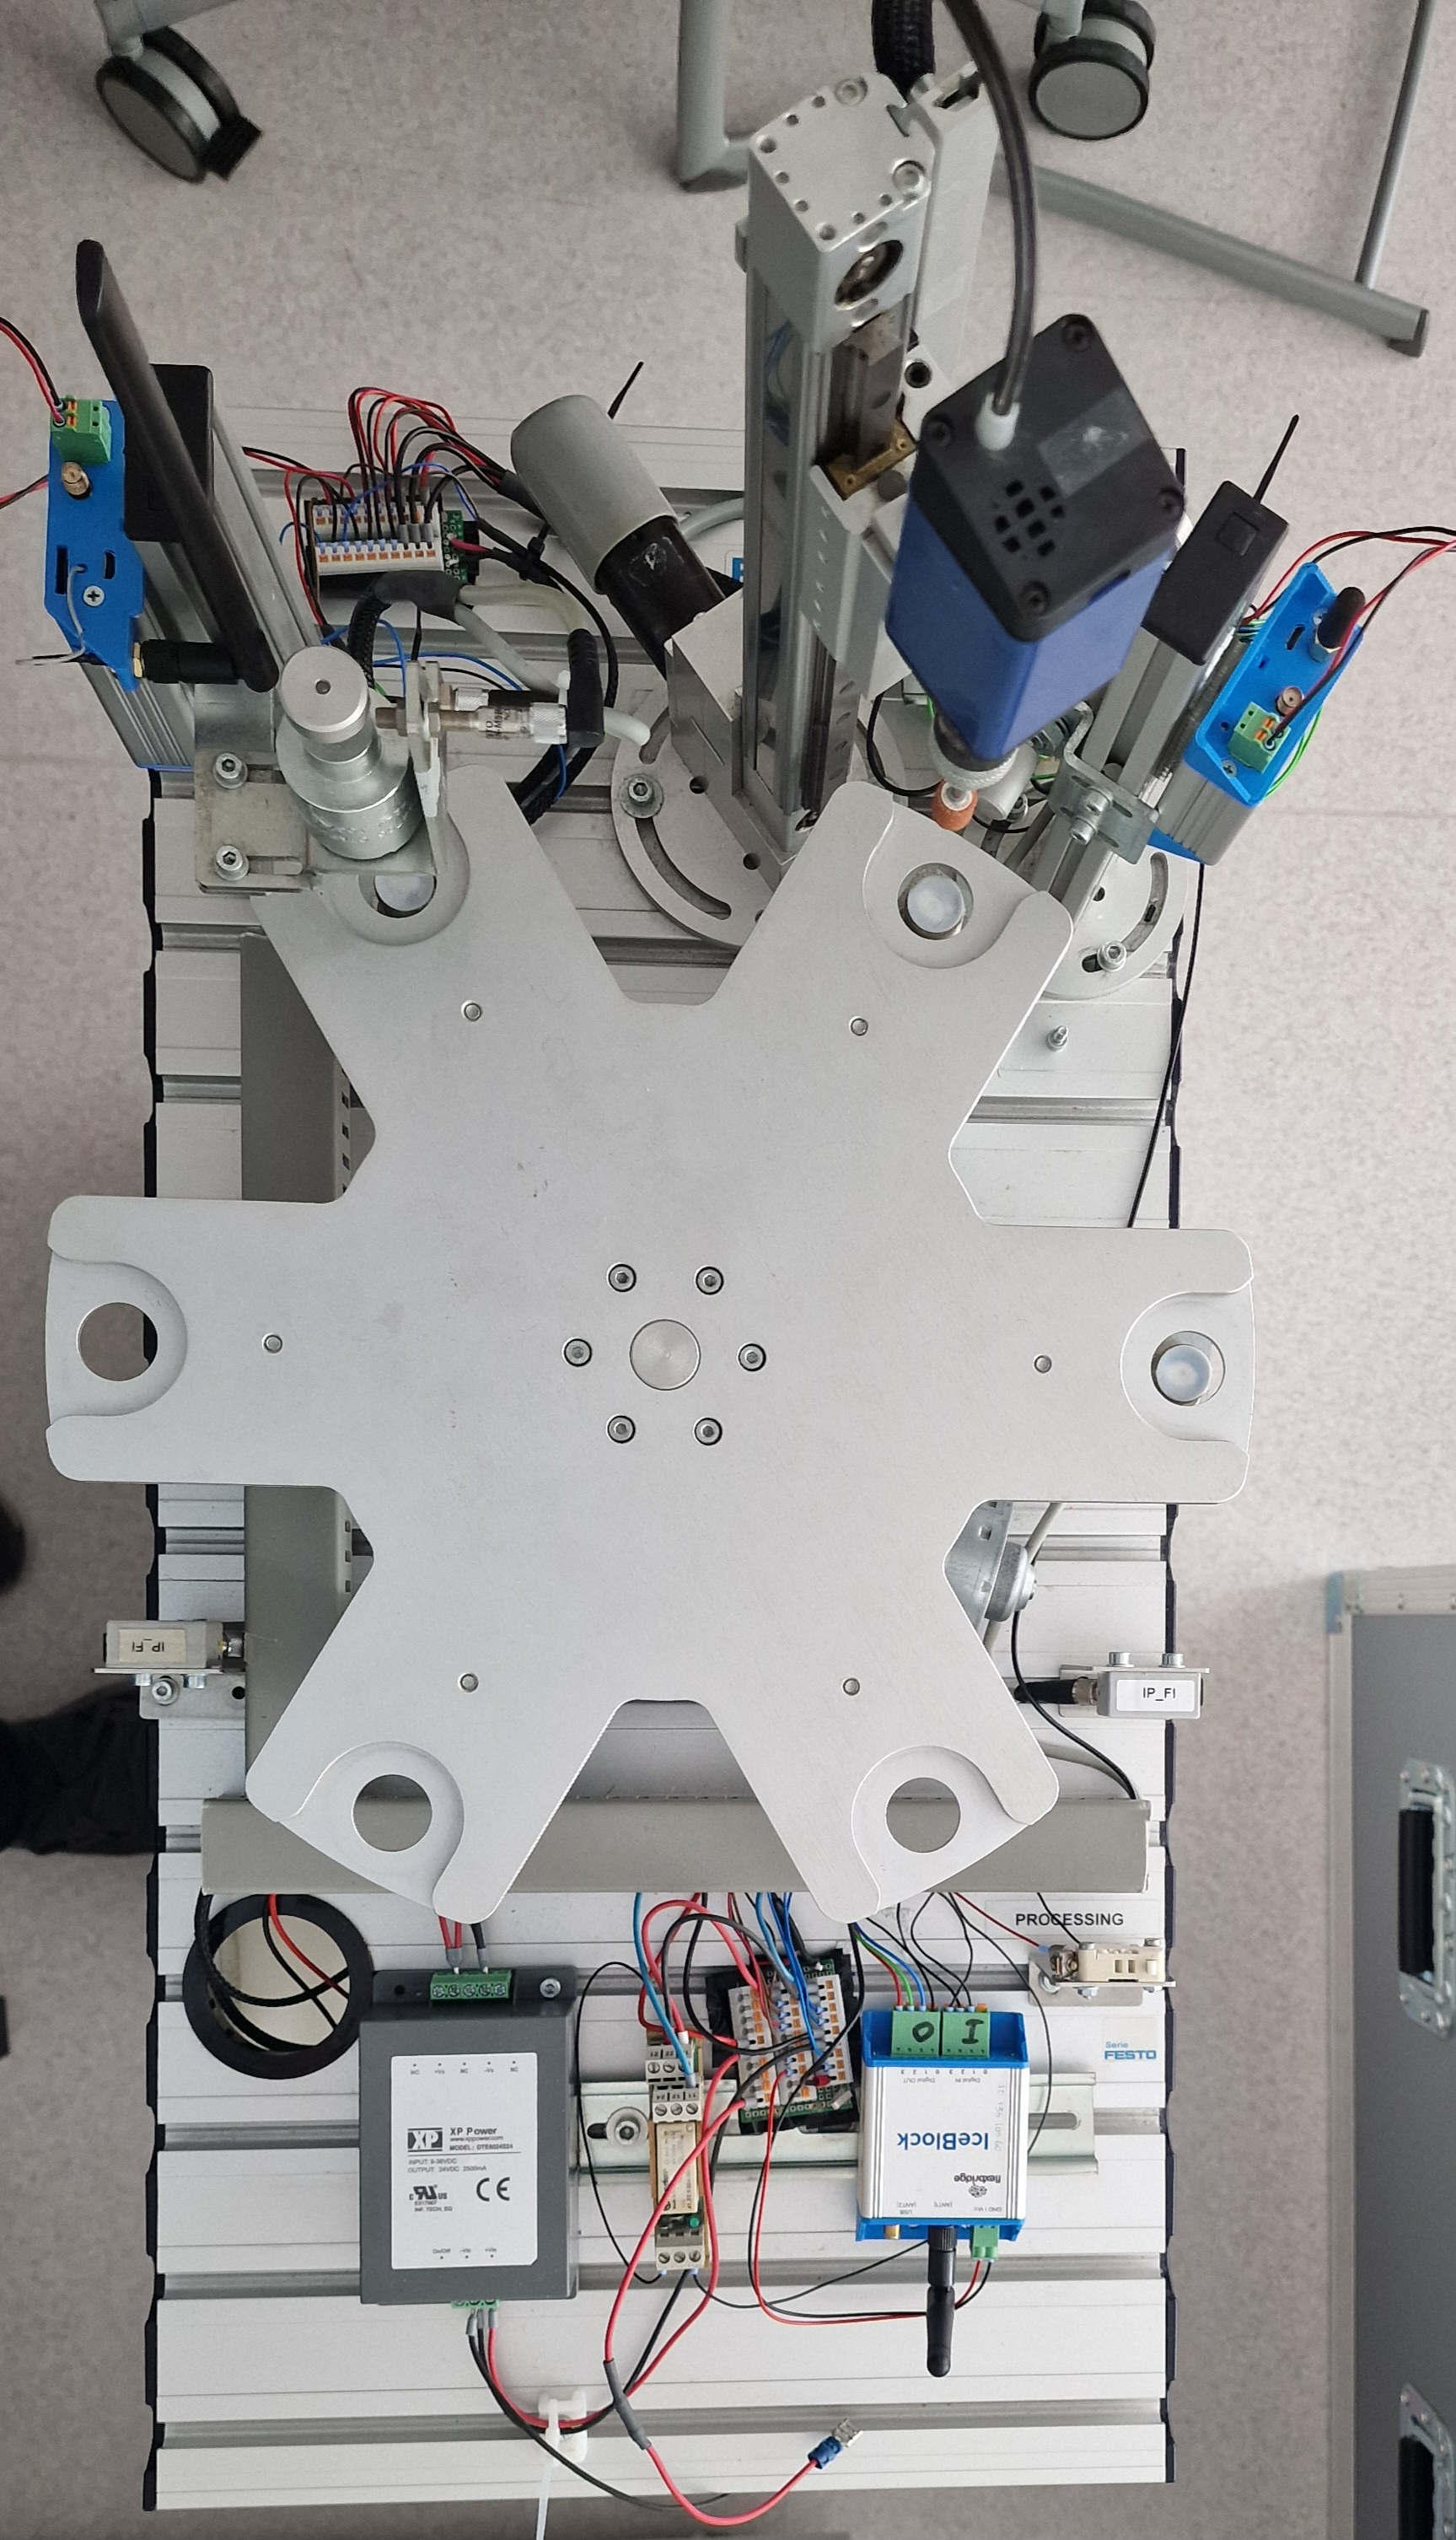
\includegraphics[width=0.5\linewidth,clip]{OJIES_2024/Figures/processingStation.jpg}
		\caption{Processing station}
		\label{fig:ps}	
 \end{figure}

The processing station system implemented in IEC~61499 is designed to control various mechatronic components through an integrated application. Each of these components is equipped with its own control device, which execute distinct control programs, i.e., the TableControl, TesterControl, and DrillControl programs. The application is implemented following the "Chain of Actions" design pattern \cite{Patil.2018}, which draws inspiration from the "Chain of Responsibility" design pattern. Each of the components is implemented as a FB network that is shown in Figure~\ref{fig:Application}. For the evaluation, three Basic FBs controlling the respective substations will be presented in detail.

\subsubsection{Table Control: Rotation}
The TableControl FB network (cf. Figure~\ref{fig:Application} \textit{top}) is responsible for rotating the table to position the material appropriately under the tester and drill components. The \texttt{WPdeliveryService} FB, a composite FB encapsulating another FB network, manages this rotation through the \texttt{TableDriver} FB and a pair of \texttt{E\_DELAY} FBs. The latter are part of the core FB library defined in the standard. Multiple instances of \texttt{WPdeliveryService} are included in the control application. 

The \texttt{TableRotate} FB encapsulates the core control logic within the network, making it the primary focus for testing the component's features. Its interface and state diagram are shown in Figure~\ref{fig:TableRotate}. The FB controls the rotational movement of a table machine which can rotate to different positions as required by the system's operation through state transitions. The primary functions include starting the rotation, monitoring the rotation process, checking if the table is in the correct position, and handling timeouts. This FB ensures that the table's motion is accurately controlled and stops when the desired position is reached or if a timeout occurs. As shown in the FB interface, the main events are \texttt{ROTATE} and \texttt{TIMEOUT\_EXCEED}. The \texttt{inPosition} input variable signals that the table has reached its target position, while output events such as \texttt{DRIVE\_ON}, \texttt{DRIVE\_OFF}, and \texttt{DONE} manage the rotation process. The state diagram (i.e., ECC) initially has an active \texttt{START} state, moves to \texttt{ROTATE\_START} when the rotation begins, and transitions to \texttt{ROTATE\_CONTINUE} if a timeout occurs. Once the table is in position, the FB transitions to \texttt{DONE}, stops the rotation, and then returns to \texttt{START}, ensuring precise control of the table's movement. Two test scenarios for the timeout are included as service sequences in Figure~\ref{fig:TableRotate}. They show that the drive is switched off if the position has been reached. The scenarios ensure that the rotation is stopped even if the signal \texttt{inPosition} is not received correctly. 
%\todo[inline]{MX: please check that the sequences (test cases) seem correct.}
\begin{figure}[bt]
	\centering
		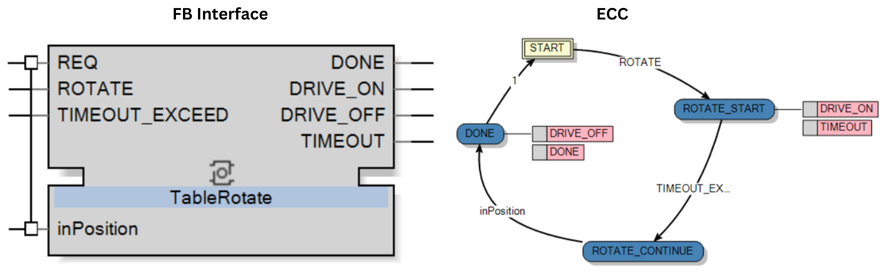
\includegraphics[width=0.99\linewidth,clip]{OJIES_2024/Figures/TableRotate.png}
            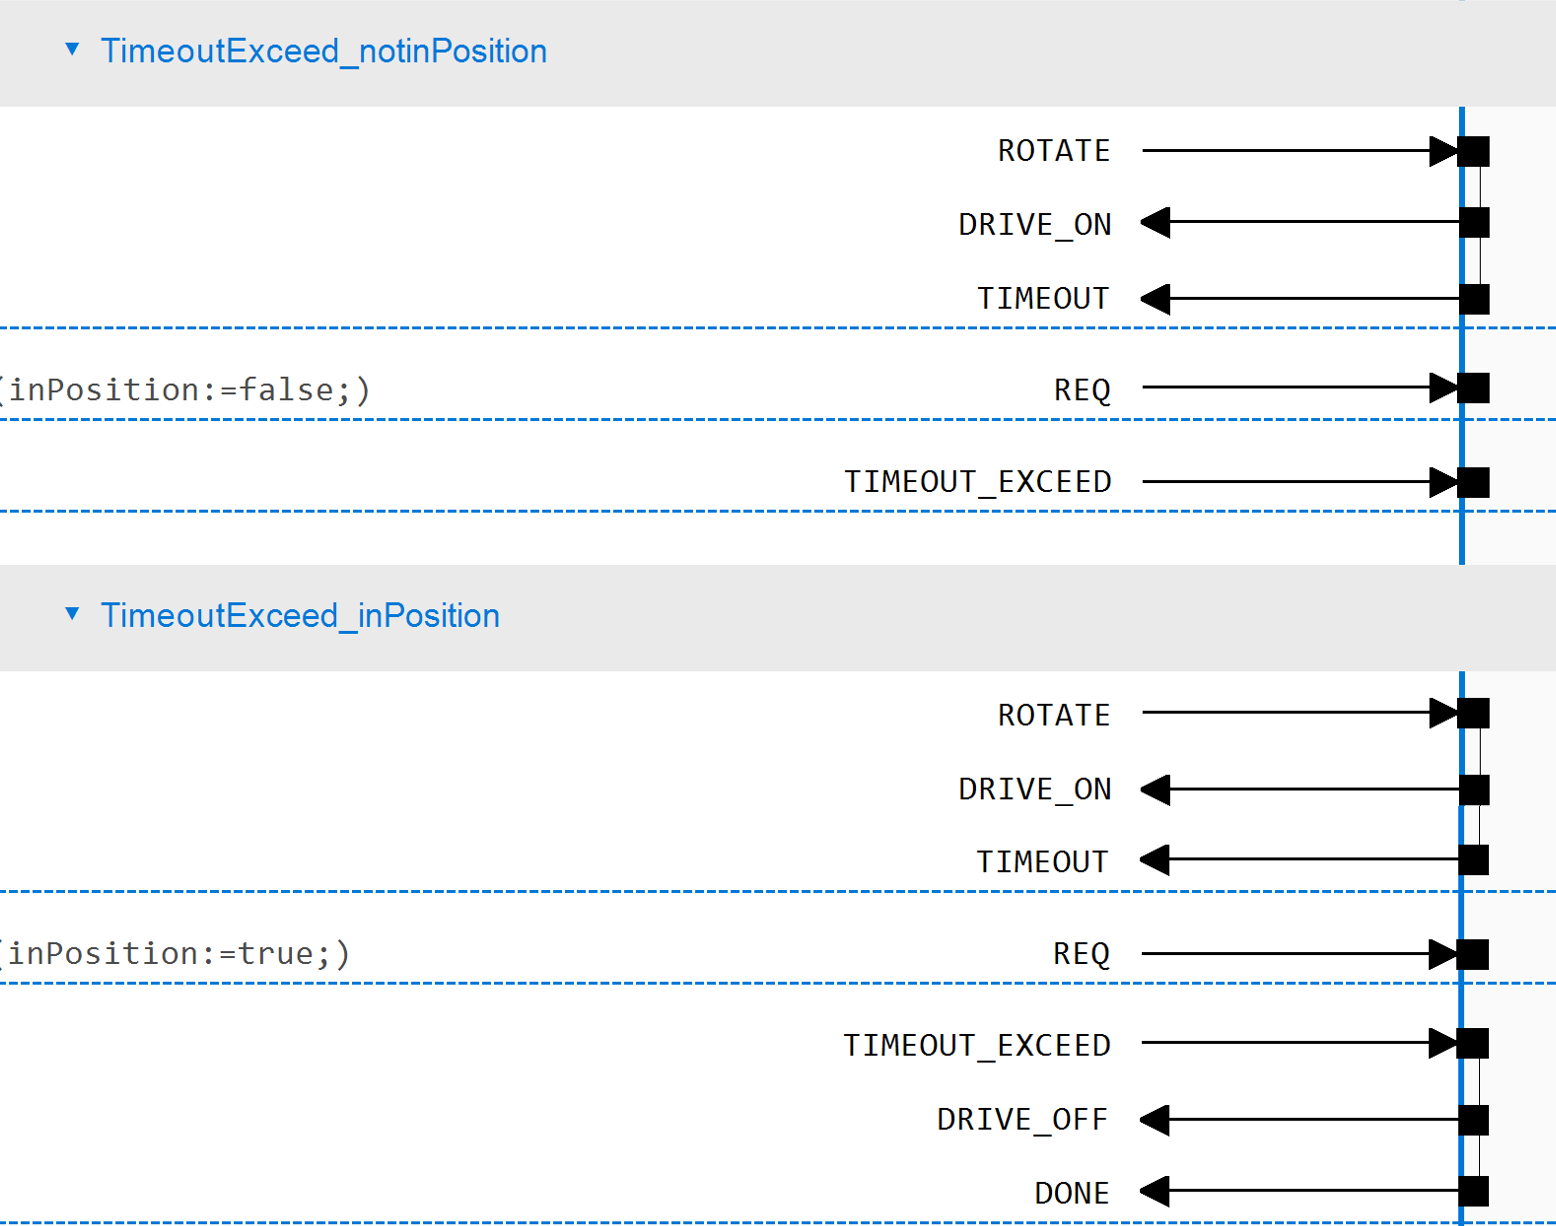
\includegraphics[width=0.99\linewidth]{OJIES_2024/Figures/tests_casestudy/Service-TableRotate_selected.png}
        \caption{TableRotate: Interface, state diagram, and selected test cases.}
		\label{fig:TableRotate}	
 \end{figure}
 \begin{figure*}[bt]
	\centering
		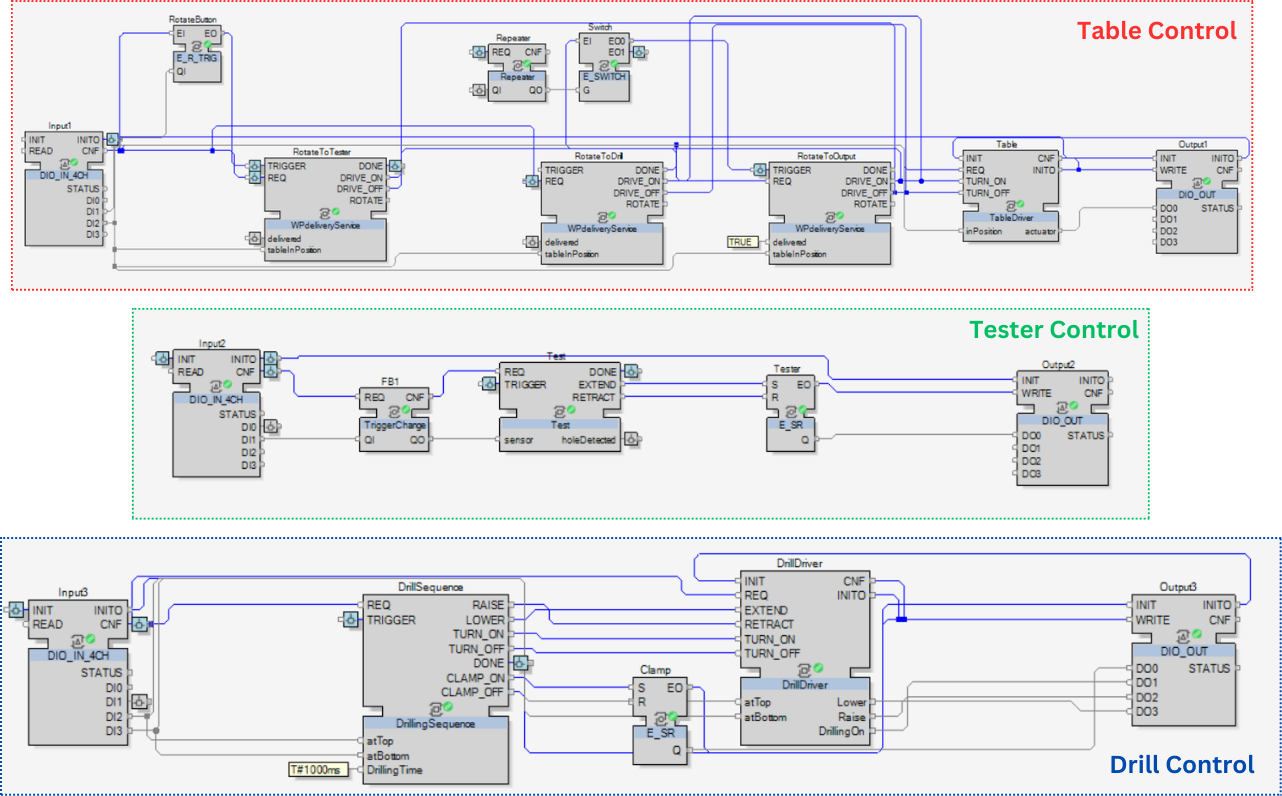
\includegraphics[width=0.99\linewidth,clip]{OJIES_2024/Figures/FB_App.png}
		\caption{Control applications for the three substations including input FBs for processing signals from the physical system, control blocks orchestrating the station, and output FBs for writing information to actuators.}
		\label{fig:Application}	
 \end{figure*}

\subsubsection{Tester Control: Inspection}
The FB network for the Tester component, TesterControl, detects holes in the workpiece to prevent that a workpiece is drilled more than once and to verify that the workpiece has undergone drilling. The main component is the Composite FB \texttt{Test} which is comprised of a standard library FB (\texttt{E\_DELAY}) and the \texttt{TestCtrl} Basic FB. 

Upon activation, the \texttt{TestCtrl} FB uses sensor data to check whether a hole is present in the workpiece. In this case, it confirms that drilling was complete. The FB manages the sequence of extending, checking, and retracting the probe, and handles timeouts in case the process takes too long. The interface and ECC of the FB are shown in Figure~\ref{fig:TestCtrl}. 
The primary input event, \texttt{TRIGGER}, initiates the detection sequence, with \texttt{QI} qualifying this event and \texttt{QO} reflecting the detection result. The FB has four output events: \texttt{EXTEND} to extend the sensor, \texttt{RETRACT} to retract it, \texttt{DONE} to signal that the process was completed, and \texttt{TIMEOUT} to initiate a timer. The ECC transitions from \texttt{START} to \texttt{EXTEND} upon receiving \texttt{TRIGGER}, and if a timeout occurs, moves to \texttt{CHECK} to determine whether a hole was detected. It then transitions to \texttt{RETRACT} and finally to \texttt{DONE}. A test case that shows the behaviour in the case of a timeout is shown in Figure~\ref{fig:TestCtrl}. 
\begin{figure}[h!]
	\centering
		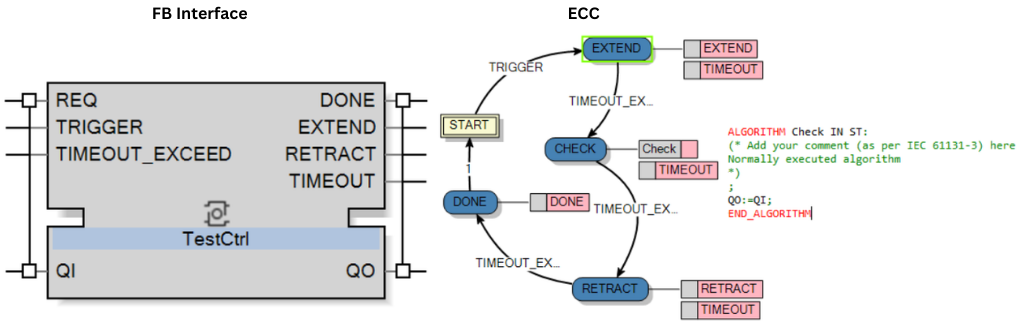
\includegraphics[width=0.99\linewidth,clip]{OJIES_2024/Figures/TestCtrl.png}
            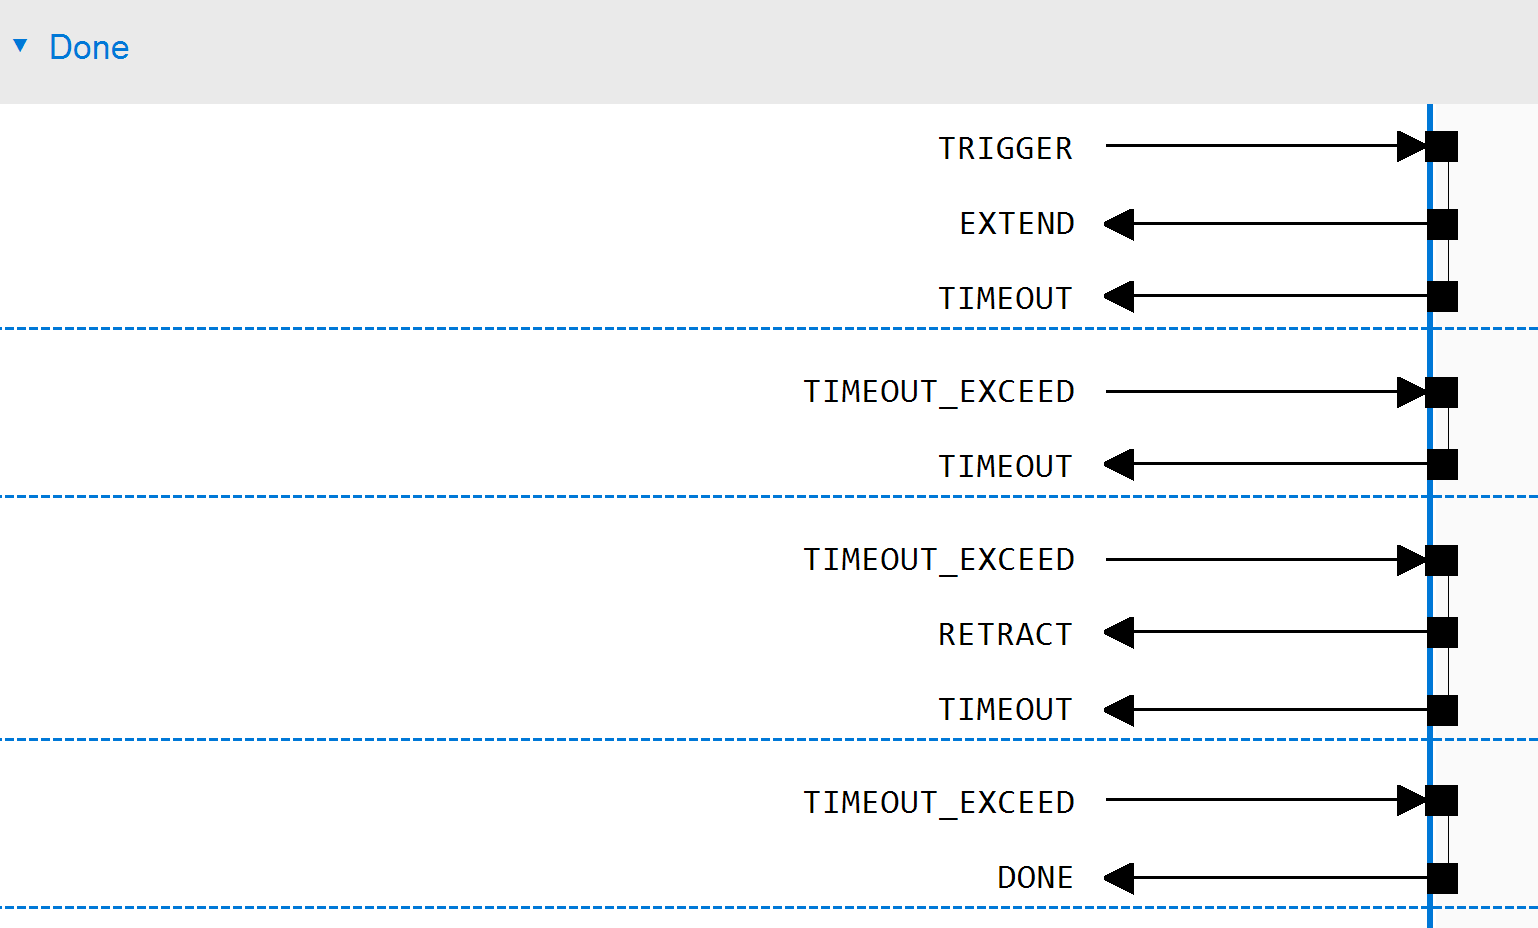
\includegraphics[width=0.99\linewidth]{OJIES_2024/Figures/tests_casestudy/Service-TestCtrl_timeout.png}
		\caption{TestCtrl: Interface, state diagram and a selected test case.}
		\label{fig:TestCtrl}	
 \end{figure}
 
\subsubsection{Drill Control: Processing}
The FB network for the drill component, DrillControl, orchestrates the drilling process. The main FBs are \texttt{DrillingSequence} and \texttt{DrillDriver}. The \texttt{DrillingSequence} is a composite FB that uses two FBs, \texttt{DoubleActingCylinder} and \texttt{SingleActingAc\-tu\-a\-tor}. The former is responsible for controlling the vertical movement of the drill, while the latter controls the rotation of the drill motor. As the \texttt{DoubleActingCylinder} FB contains the core logic of the drilling process, it is shown in Figure~\ref{fig:DoubleActingCylinder}. It controls the bidirectional motion of a drill machine, specifically managing its upward and downward movements. This control is essential for operating machinery that uses linear actuators, such as hydraulic or pneumatic cylinders, to extend and retract, corresponding to the downstroke and upstroke of the drill. The FB handles initialization, execution requests, extension (downward movement), and retraction (upward movement), with input conditions determining the cylinder's state transitions and output commands controlling the actuators.
Specifically, the cylinder movement is controlled via the events \texttt{EXTEND} and \texttt{RETRACT}. The input variables \texttt{atHome} and \texttt{atEnd} indicate the cylinder's position, while the output variables \texttt{extend} and \texttt{retract} command its motion. The ECC %manages transitions between states (\texttt{HOME}, \texttt{EXTEND}, \texttt{END}, and \texttt{RETRACT}), 
ensures that the cylinder moves correctly based on events and position feedback. The algorithms activate or stop the cylinder's movement, ensuring precise control for upward and downward motion. 
\begin{figure}[hbt]
	\centering
		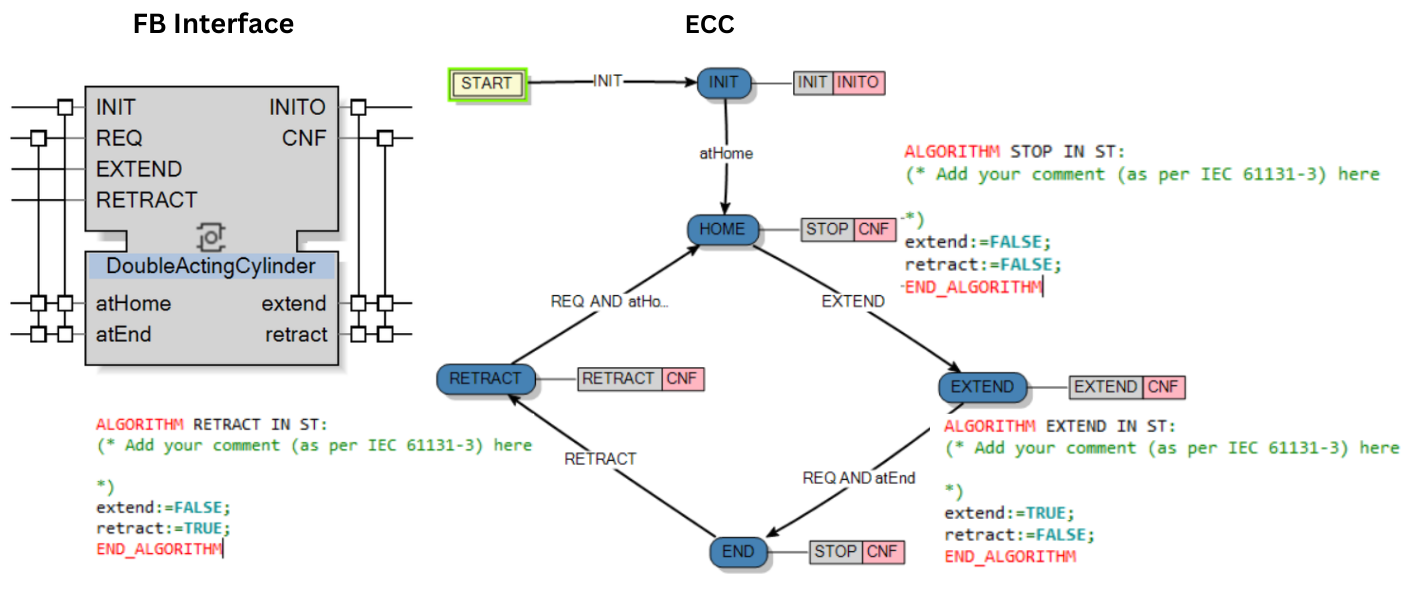
\includegraphics[width=0.99\linewidth,clip]{OJIES_2024/Figures/DoubleActingCylinderV2.png}
            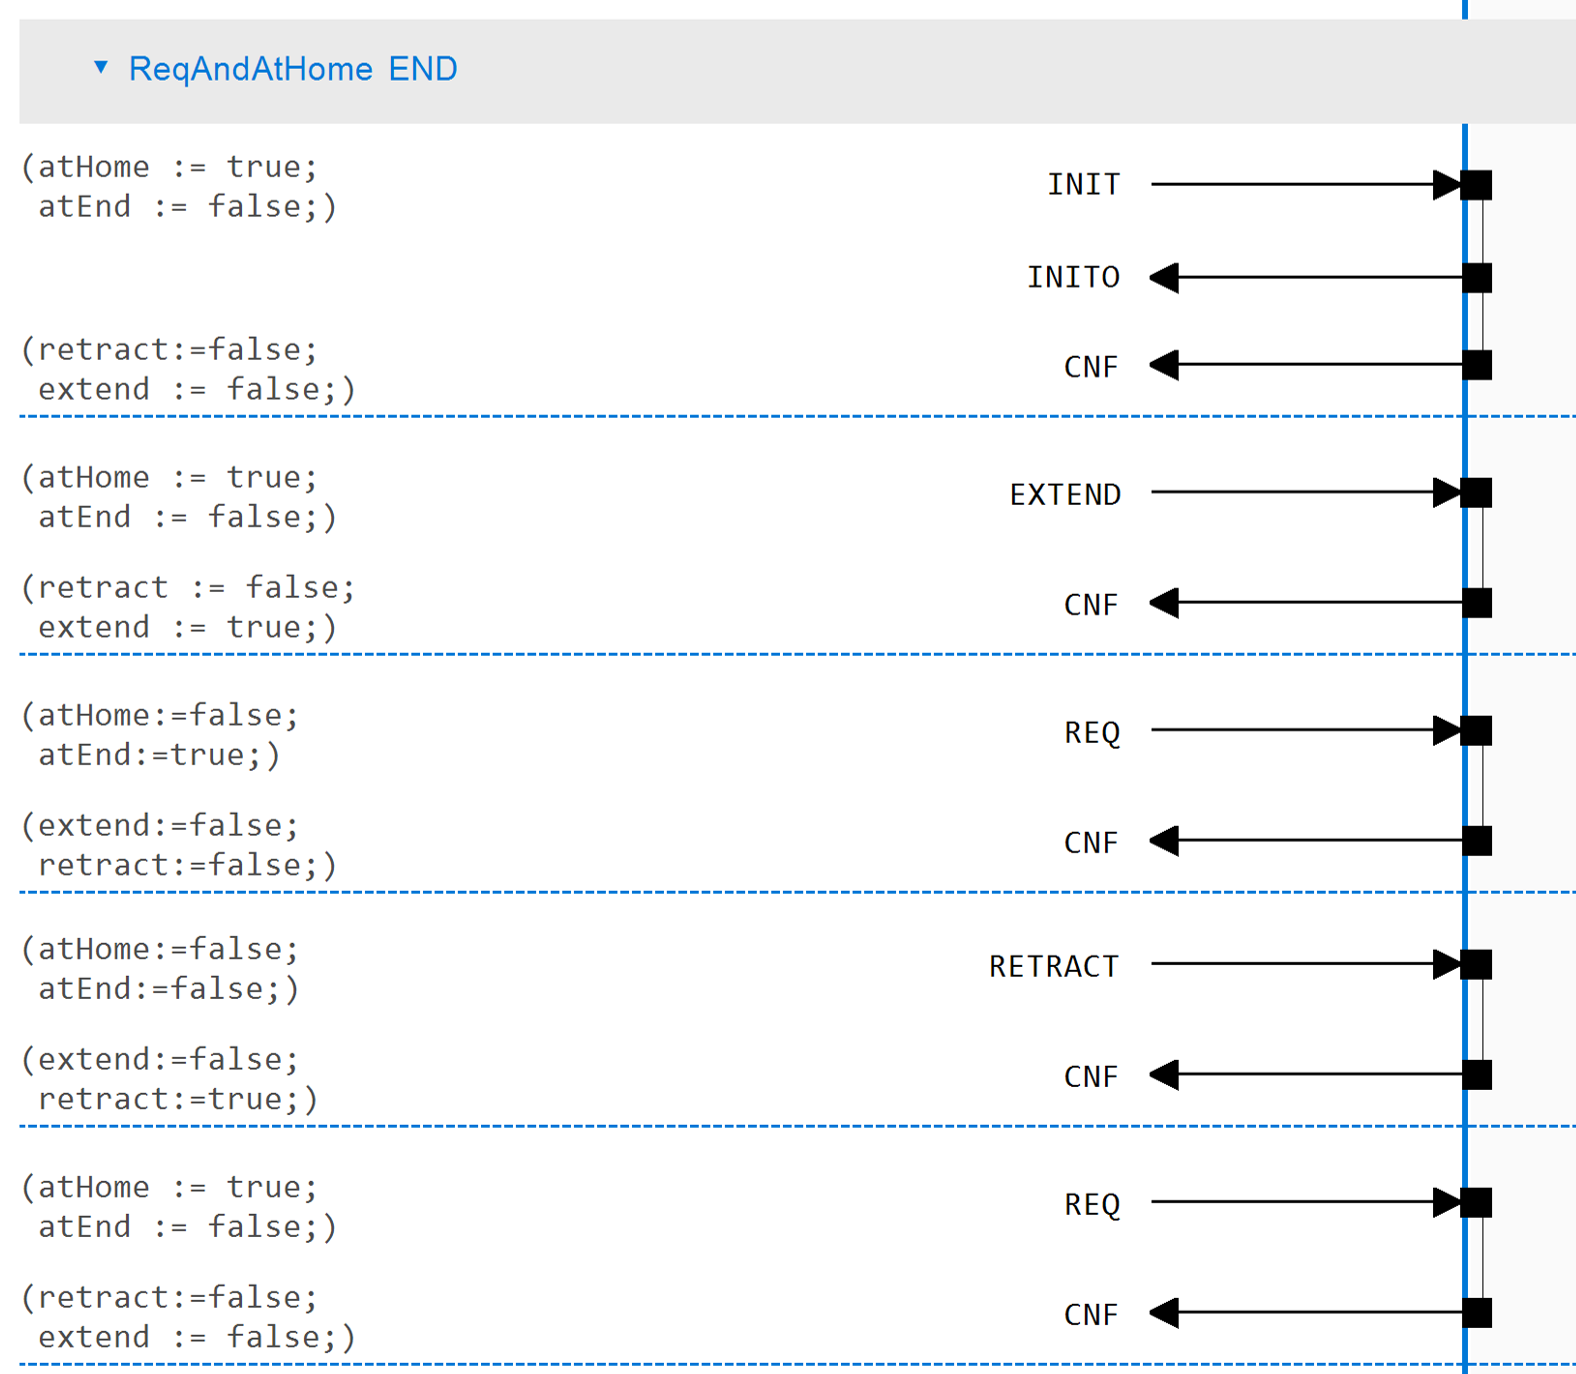
\includegraphics[width=0.99\linewidth]{OJIES_2024/Figures/Service-DoubleActingCylinder_selected.png}
		\caption{Double Acting Cylinder: Interface, state diagram, and selected test cases}
		\label{fig:DoubleActingCylinder}	
 \end{figure}

\section{Evaluation}
We tested the main control FBs from the processing station, but also validated the implementation itself. Following our methodology, we imported any FBs from other tools into 4diac IDE. In 4diac IDE, we then generated the test application, which was executed in 4diac~FORTE and in EcoRT.

\subsection{Evaluating the Generation Framework in Eclipse 4diac}
Selected test cases defined as service sequences as shown in Figures~\ref{fig:TableRotate}, \ref{fig:TestCtrl} and \ref{fig:DoubleActingCylinder}. In total, 12 test cases were created which described both the expected interactions with an FB and deviations (such as events from the environment that occur in a reversed order). To additionally validate that the framework can successfully detect failed test cases, we intentionally defined five service sequences with unexpected behaviour. An example for the TableRotate FB is shown in Figure~\ref{fig:table_rotate_fail}. These experiments validate that the generated test application can indeed detect deviations between the implementation and the specification.

\begin{figure}[hbt]
    \centering
    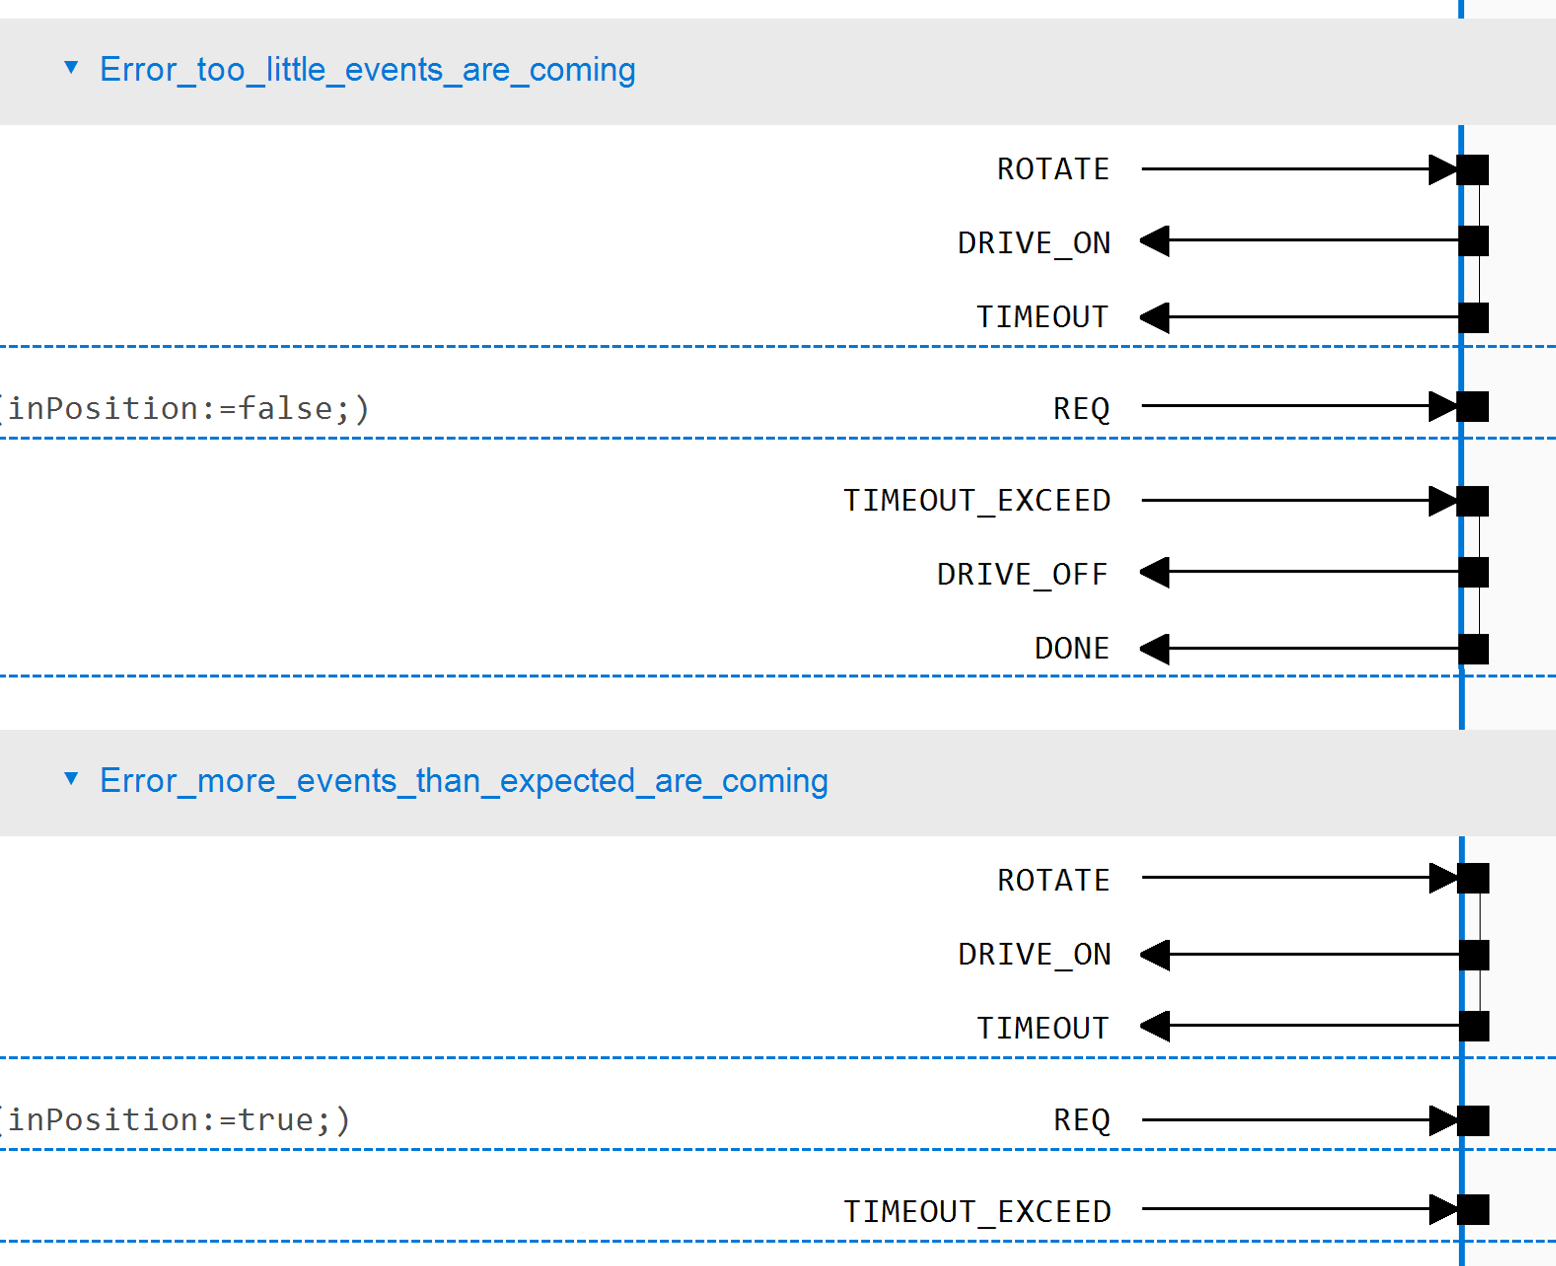
\includegraphics[width=0.7\linewidth]{OJIES_2024/Figures/tests_casestudy/Service-TableRotate_negative.png}
    \caption{Service sequences that result in failed test cases for a correct implementation.}
    \label{fig:table_rotate_fail}
\end{figure}


%We imported the FBs to Eclipse 4diac, defined the tests in its IDE, and generated test applications for them. We also executed the test application on the accompanying runtime 4diac FORTE. After porting the test application to EcoStruxure, we also executed the tests on their runtime environment.

\begin{comment}
\subsubsection{Test case definitions}
Double-acting cylinder
- when it is at home: EXTEND  -> instead of accidentally retract

TestCtrl
- forget to check the sensor value in the ECC

TableRotate
- rotating on/off
- if rotating does not stop after some time, we have a problem (signal inPosition not received -> then it does not stop rotating)
- real example: if you forget to turn a little, the sensor value does not get update


- specify test cases
- introduce faults!?
- try to detect faults with the specified test cases
- report results
\end{comment}

\begin{figure}[h!]
	\centering
		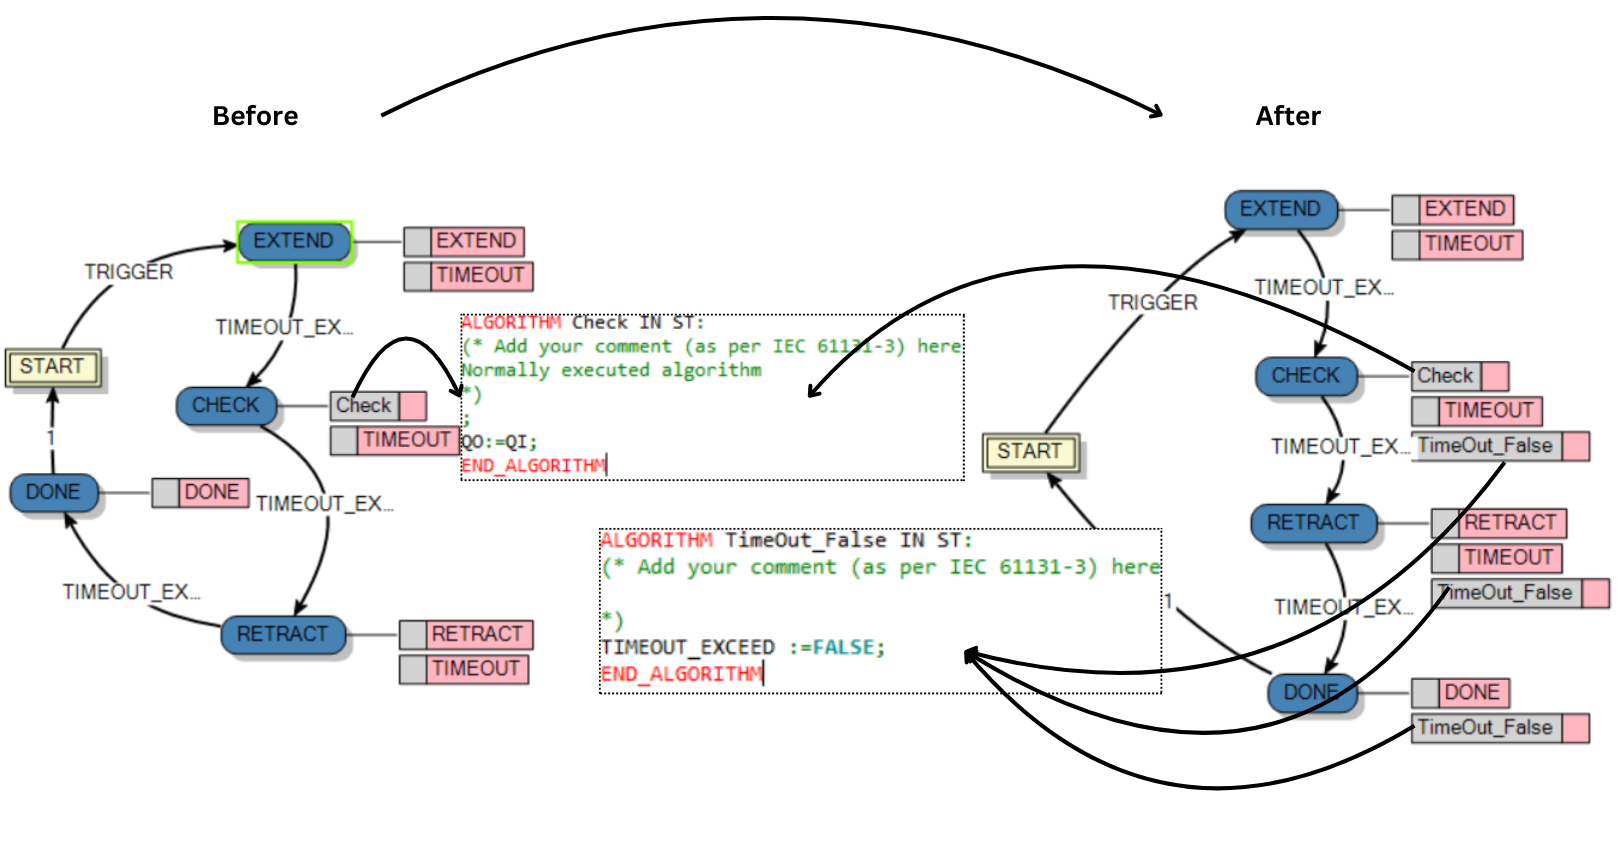
\includegraphics[width=0.99\linewidth,clip]{OJIES_2024/Figures/SemanticExexcissue.png}
		\caption{Semantic Execution issue}
		\label{fig:SemanticExexcissue}	
 \end{figure}

\subsection{Semantic Variants in Ported Software}
All involved FBs were manually imported in a second tool environment to evaluate the behavior of a ported test application. Unfortunately, the testing of FBs on the EcoStruxure Automation Expert (EAE) revealed that certain test cases were failing when executed on the Tester Control. Modifications to the framework were required to compensate the variations in the implemented execution semantics.

Upon thorough analysis, it was determined that these failures were attributed to a semantic execution issue inherent in the EAE. Unlike specified the IEC 61499 standard, EAE adopts a specific semantic execution model. This divergence in execution semantics implies that when a real-world application is ported from Eclipse 4diac to EAE, it may not function correctly, and in some cases, it may even result in system failures.

EAE's semantic execution model operates such that when two or more identical events are used as a sequence of events to transition through multiple states, a single event trigger results in a direct transition to the final state. Specifically, when the event triggers once, the system bypasses intermediate states and directly reaches the final state. 
To illustrate this issue, consider the ECC shown in Figure~\ref{fig:SemanticExexcissue} where the event \texttt{TIMEOUT\_EXCEEDED} is expected to facilitate a sequence of state transitions. According to the desired behavior, upon the first occurrence of the \texttt{TIMEOUT\_EXCEEDED} event, the system should transition to a state labeled \texttt{CHECK}. It should remain in this \texttt{CHECK} state, awaiting a subsequent \texttt{TIMEOUT\_EXCEEDED} event to be triggered before progressing to the final state labeled \texttt{DONE}. However, due to the semantic execution model employed by EAE, when the \texttt{TIMEOUT\_EXCEEDED} event is triggered only once, the system bypasses the \texttt{CHECK} state entirely and directly transitions to the \texttt{DONE} state. This behavior deviates from the intended design, leading to incorrect execution flow.

To address this issue, the test case generation framework was modified to compensate the semantic execution differences. This algorithm modifies the \texttt{TIMEOUT\_EXCEEDED} event by setting its value to \texttt{FALSE}, ensuring that the system remains in the \texttt{CHECK} state after the initial trigger. Consequently, the system only moves to the next state when a subsequent \texttt{TIMEOUT\_EXCEEDED} event is triggered. This modification aligns the execution flow with the expected sequence, preventing premature transitions to the final state.



\section{Results and Discussion}
\label{sec::results}
The semantic differences outlined in the previous section demonstrate the need for a cross-platform testing framework. While the semantic differences could be bridged within our implemented generators, transferring real-world FBs between execution environments can lead to undetected failures. In any portability scenario, this would mean that the distribution of software parts across various vendor's IDEs introduces bugs that are difficult to detect.

It was observed that the control application for our demonstrator contained certain bugs after porting to Eclipse 4diac, which were uncovered during the execution of the test cases. These issues highlight the importance of recognizing the semantic execution differences between EAE and the IEC 61499 standard when porting applications. Addressing such discrepancies is crucial to ensure that applications function as intended within the EAE environment.

The migration of Function Blocks (FBs) from Eclipse 4diac to EcoStruxure Automation Expert (EAE) presents several challenges. Initially, the FBs were imported into 4diac IDE, where tests were defined and test applications were generated. 
These test applications were executed on the accompanying runtime environment, 4diac FORTE. However, when these test applications were ported to EcoStruxure and executed on the EcoRT runtime environment, portability issues arose. The following outlines the key challenges encountered during this migration process.

One significant challenge involves the direct addition of a composite FB containing the \texttt{E\_DELAY} FB. The \texttt{E\_DELAY} FB is a standard function block that is pre-compiled into the vendor's runtime environment. Due to this pre-compiled nature, adding any standard FB directly is not possible. Standard FBs are already available within the vendor's IDE, which necessitates a replacement approach to ensure proper functionality. Consequently, when a composite FB that contains a standard FB is added, it becomes necessary to manually replace the standard FB with an equivalent vendor-provided standard FB within the vendor's IDE. %This manual intervention is crucial to address compatibility issues and ensure seamless integration.

Another issue encountered pertains to adapters and namespaces. In EAE, an adapter cannot be located unless the correct namespace is specified as \texttt{Main}. The definition of the appropriate namespace is essential; otherwise, the adapter will not be displayed. Correcting the namespace can resolve this particular issue. However, even after setting the correct namespace, the use of adapters in composite FBs poses additional problems. These problems require the removal and subsequent redrawing of connections, indicating that the mere correction of namespaces is insufficient when dealing with composite FBs involving adapters.

Further challenges were identified while porting the test FBs in EAE, particularly in relation to the algorithm section within the \texttt{.fbt} file. It was observed that the \texttt{start\_algorithm} and \texttt{end\_algorithm} statements were repeated twice. This redundancy results in errors that must be rectified manually by removing the duplicate statements. Additionally, case sensitivity issues arise within the algorithms. For instance, Boolean variable values are written as \texttt{"false"} and \texttt{"true"} instead of the expected \texttt{"FALSE"} and \texttt{"TRUE"}. This discrepancy requires manual correction to conform to the syntax standards of the target environment.

Another issue relates to the naming conventions used in algorithms. Algorithm names containing double underscores (\texttt{\_\_}) are not supported. As a result, any algorithm names with double underscores must be modified to eliminate this character sequence. This change is necessary to ensure that the algorithms are compatible with the EAE environment. These migration challenges highlight the need for some manual adjustments to ensure the successful transfer and execution of FBs within different automation environments.

\begin{comment}
\begin{table*}[h]
\centering
\begin{tabular}{|l|l|l|l|}
\hline
\textbf{Issue} & \textbf{EAE} & \textbf{4Diac} & \textbf{IEC 61499 Standard} \\ \hline
Direct addition of the \texttt{E\_DELAY} FB is not possible. (Migrating composite FBs with Standard FBs is complex.) & & & \\ \hline
The adapter cannot be found due to the required namespace selection as "Main." & & & \\ \hline
Repeated algorithm definitions and \texttt{end\_algorithm} statements. & & & \\ \hline
Case sensitivity issues in algorithms, e.g., "false" should be "FALSE" and "true" should be "TRUE." & & & \\ \hline
Algorithm names containing double underscores present problems. & & & \\ \hline
The use of "Main::" is not permitted. The namespace should be specified as "Main." & & & \\ \hline
Adapter connection issues require removal and redrawing of connections. & & & \\ \hline
Issues with semantic execution. & & & \\ \hline
Algorithm names containing double underscores present problems, so I changed the names. & & & \\ \hline
\texttt{timeout=false} is written in algorithms. & & & \\ \hline
\end{tabular}
\caption{Migration challenges encountered when transferring Function Blocks (FBs) from 4diac to EAE}
\end{table*}

\subsubsection{other findings}
Did we find any bugs?
Effort reduction?
Problems with different runtimes?
Problems with migration (execution semantics, XML specification)


\end{comment}

In summary, the proposed framework can reduce the effort of porting libraries because the test execution is automated rather than requiring manual labour. 

